\documentclass[11pt]{beamer}
\usetheme{CambridgeUS}

\usepackage[utf8]{inputenc}
\usepackage[english]{babel}
\usepackage{amsmath}
\usepackage{amsfonts}
\usepackage{amssymb}
\usepackage{graphicx}

\author{Jonathan Sidi}
\title[Election Analysis]{Real Time Tracking and Analysis of \\ Election Polling in Israel}
%\subtitle{}
%\logo{}
\institute[HUJI Statistics]{Department of Statistics, Hebrew University of Jerusalem}
\date{May 28, 2015}
%\subject{}
%\setbeamercovered{transparent}
%\setbeamertemplate{navigation symbols}{}

\begin{document}
\maketitle

\begin{frame}
\begin{block}{}
An R based open source web application which gathers continuously updated election polling information to one interactive location
\end{block}

\vspace{1cm}

\centering
Free, Simple, Transparent
\end{frame}

\section{Quickview}
\begin{frame}{Stay Up To Date}
\begin{block}{}
Stay up to date with latest polling results from all the pollsters
\end{block}
				\begin{figure}[h]
				\centering
				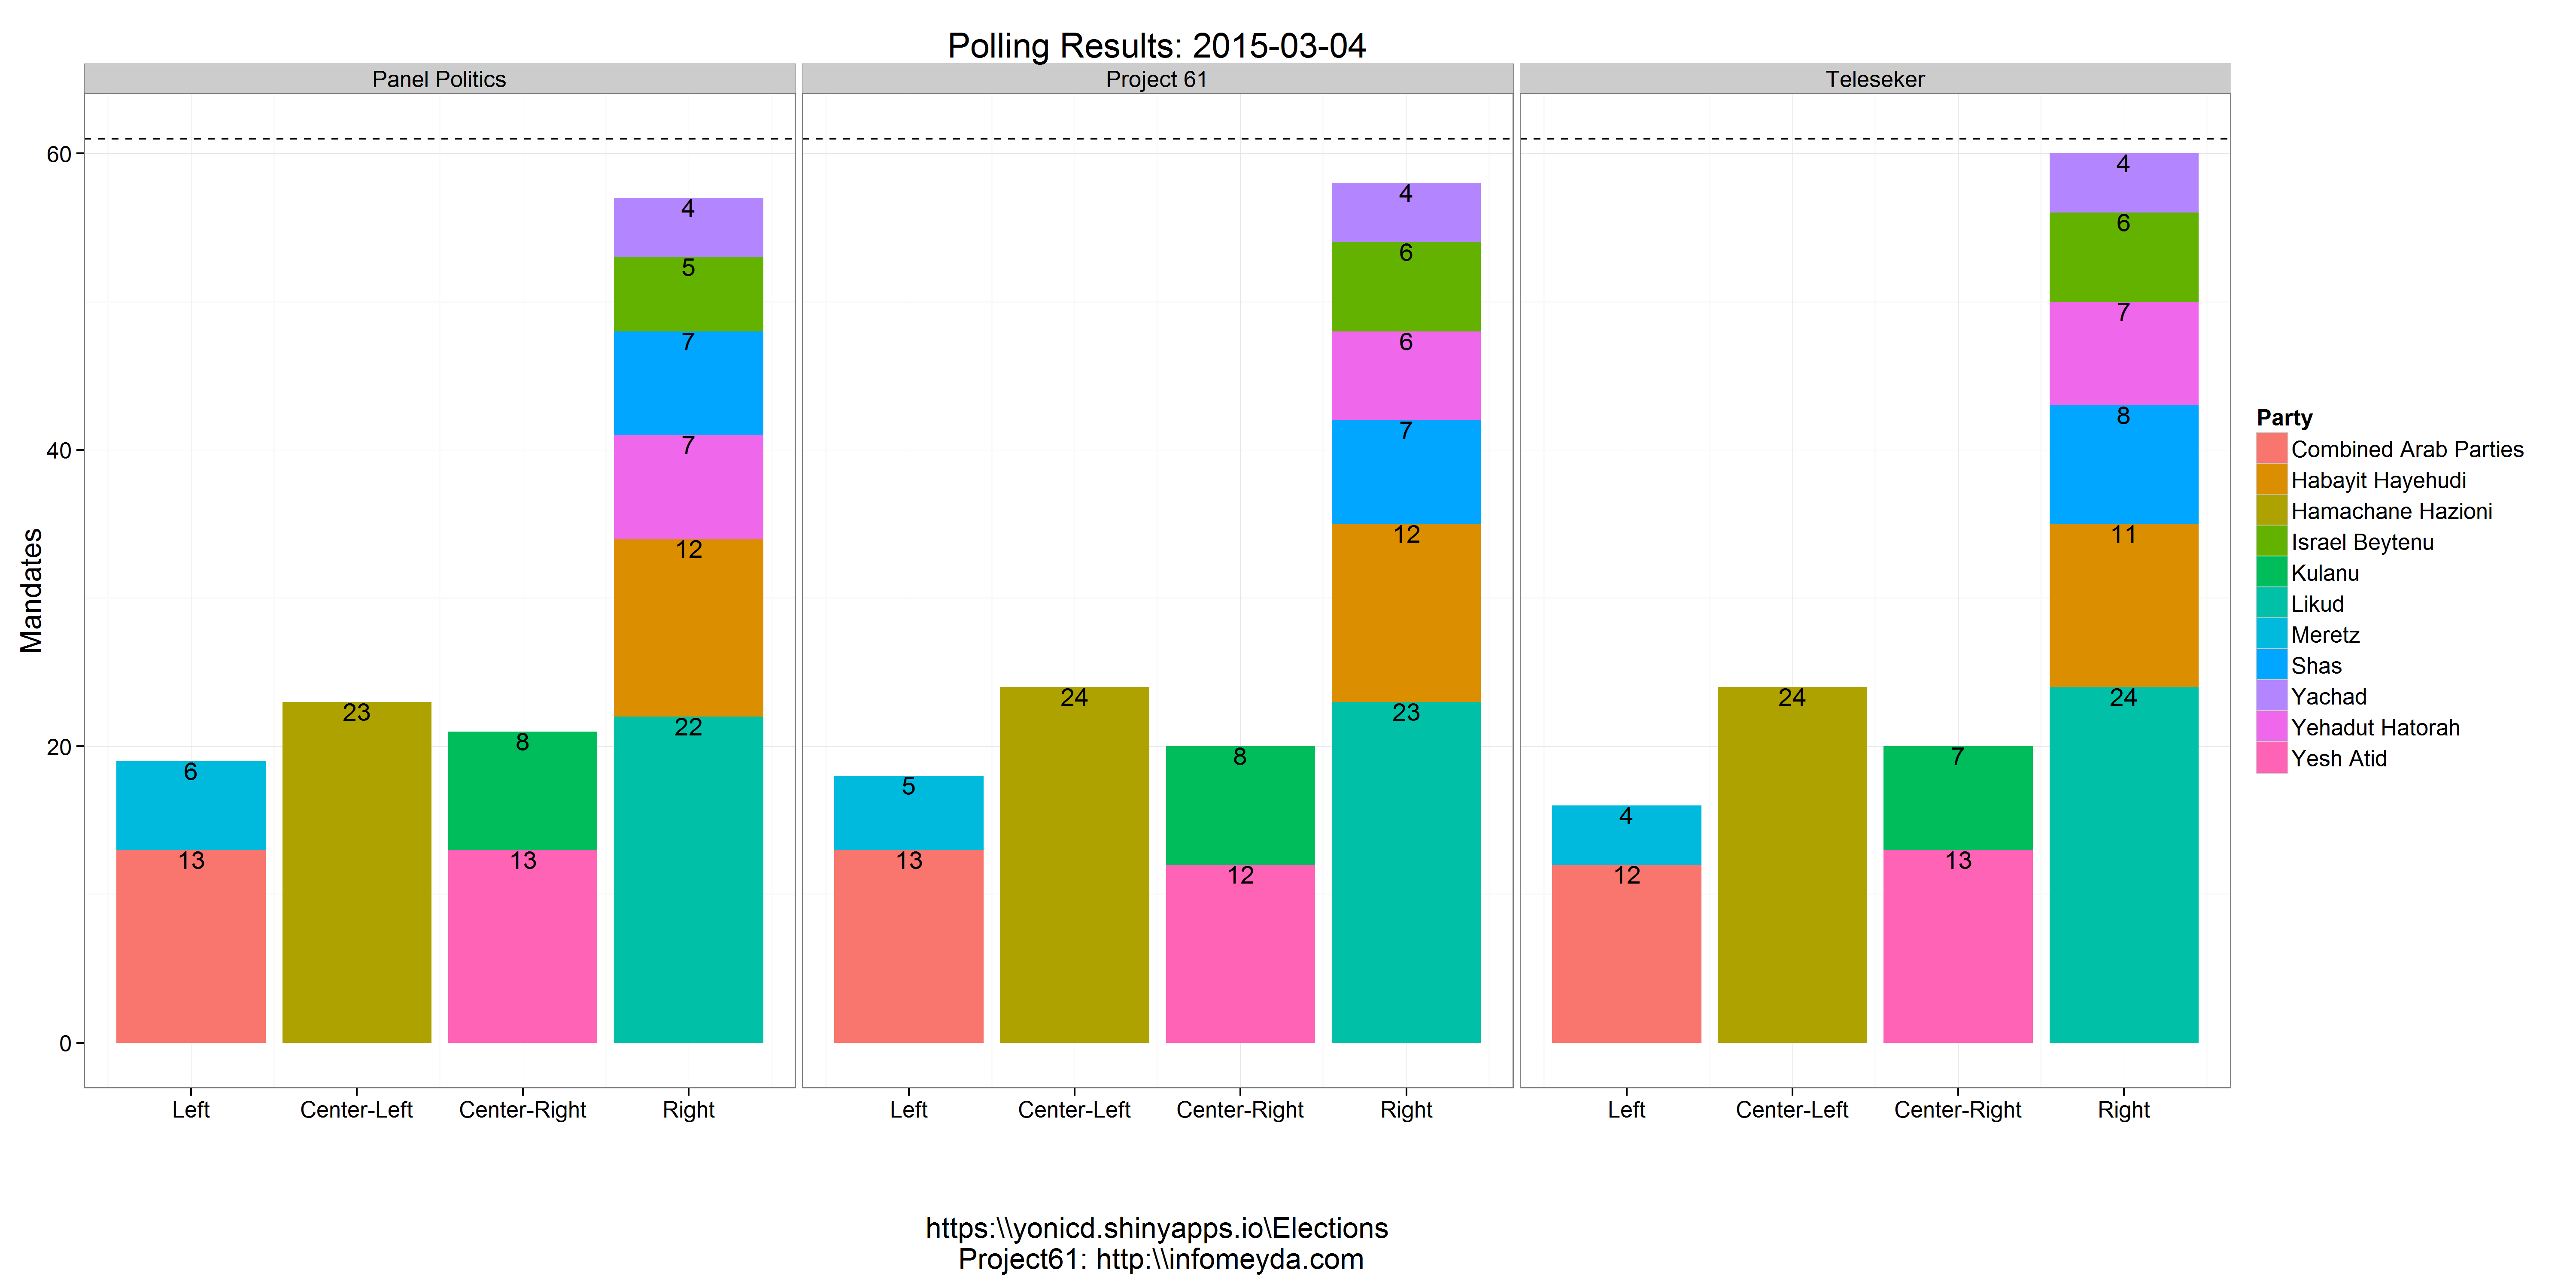
\includegraphics[width=1\linewidth]{../www/LastDayPlot}
				\label{fig:LastDayPlot}
				\end{figure}
\end{frame}

\section{Interactive}
\begin{frame}{Interactive Graphs}
\begin{columns}
\begin{column}{.4\linewidth}
\begin{itemize}
\item Trends of Party/Block
\item Drill Down
\end{itemize}
\end{column}
\begin{column}{.6\linewidth}
\begin{itemize}
\item Nested: Pollsters within Party
\item Longitudinal: Party Across Elections
\end{itemize}
\end{column}
\end{columns}



				\begin{figure}[h]
					\centering
					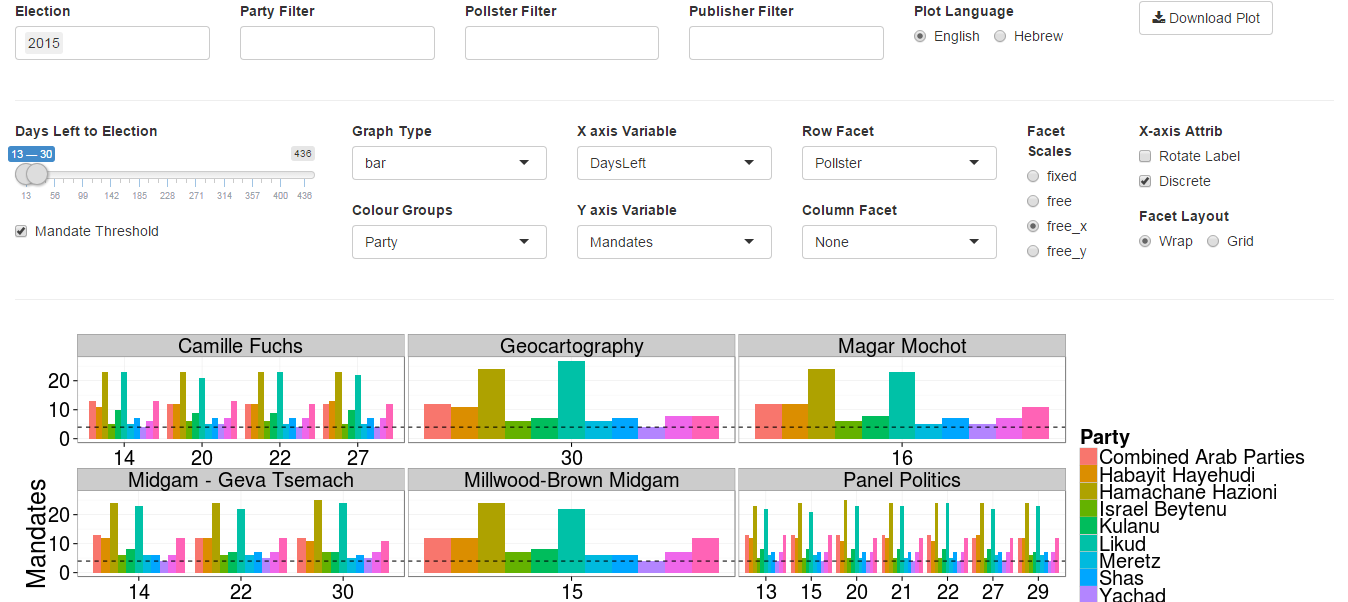
\includegraphics[width=.85\linewidth]{../www/pad_screen_grab}
					\label{fig:pad_screen_grab}
				\end{figure}

\end{frame}

%\subsection{Cross Section}
%\begin{frame}{Example: Cross Section Analysis}
%				\begin{figure}[h]
%					\centering
%					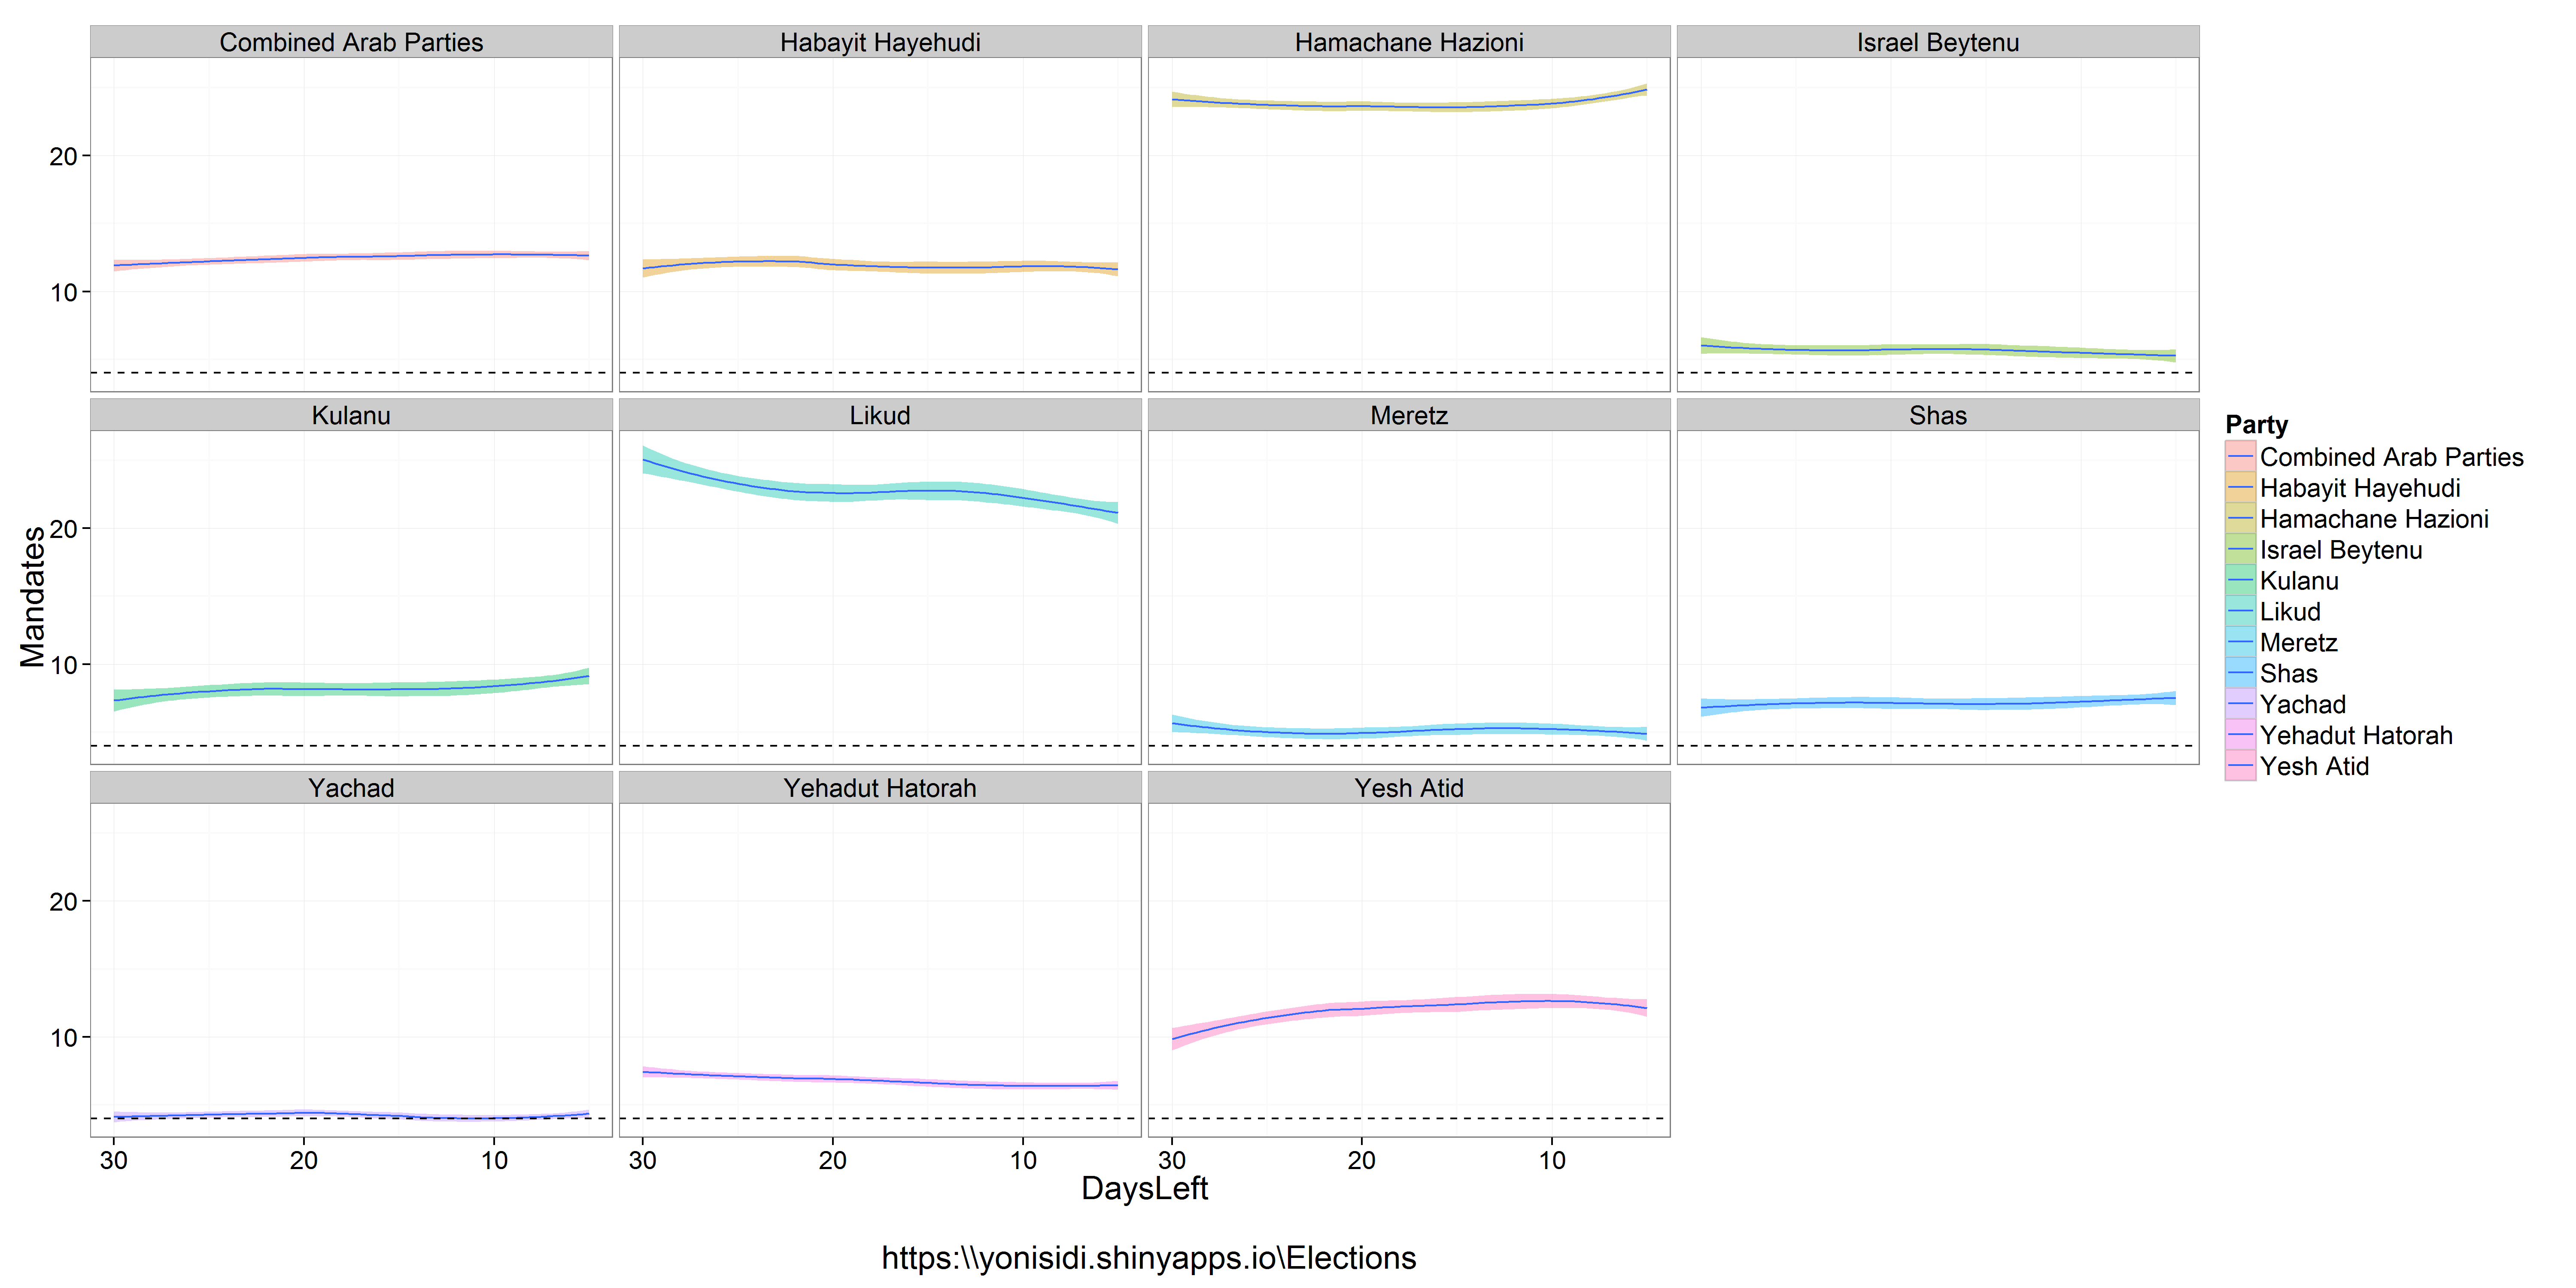
\includegraphics[width=1\linewidth]{../www/ElectionPlot_trend}
%					\label{fig:ElectionPlot_trend}
%				\end{figure}
%\begin{block}{}
%Comparison of pollster results within parties to find public sentiment variability and pollster estimation bias
%\end{block}				
%\end{frame}				
%
%\subsection{Longitudinal}
%\begin{frame}{Example: Longitudintal Analysis}				
%				\begin{figure}[h]
%					\centering
%					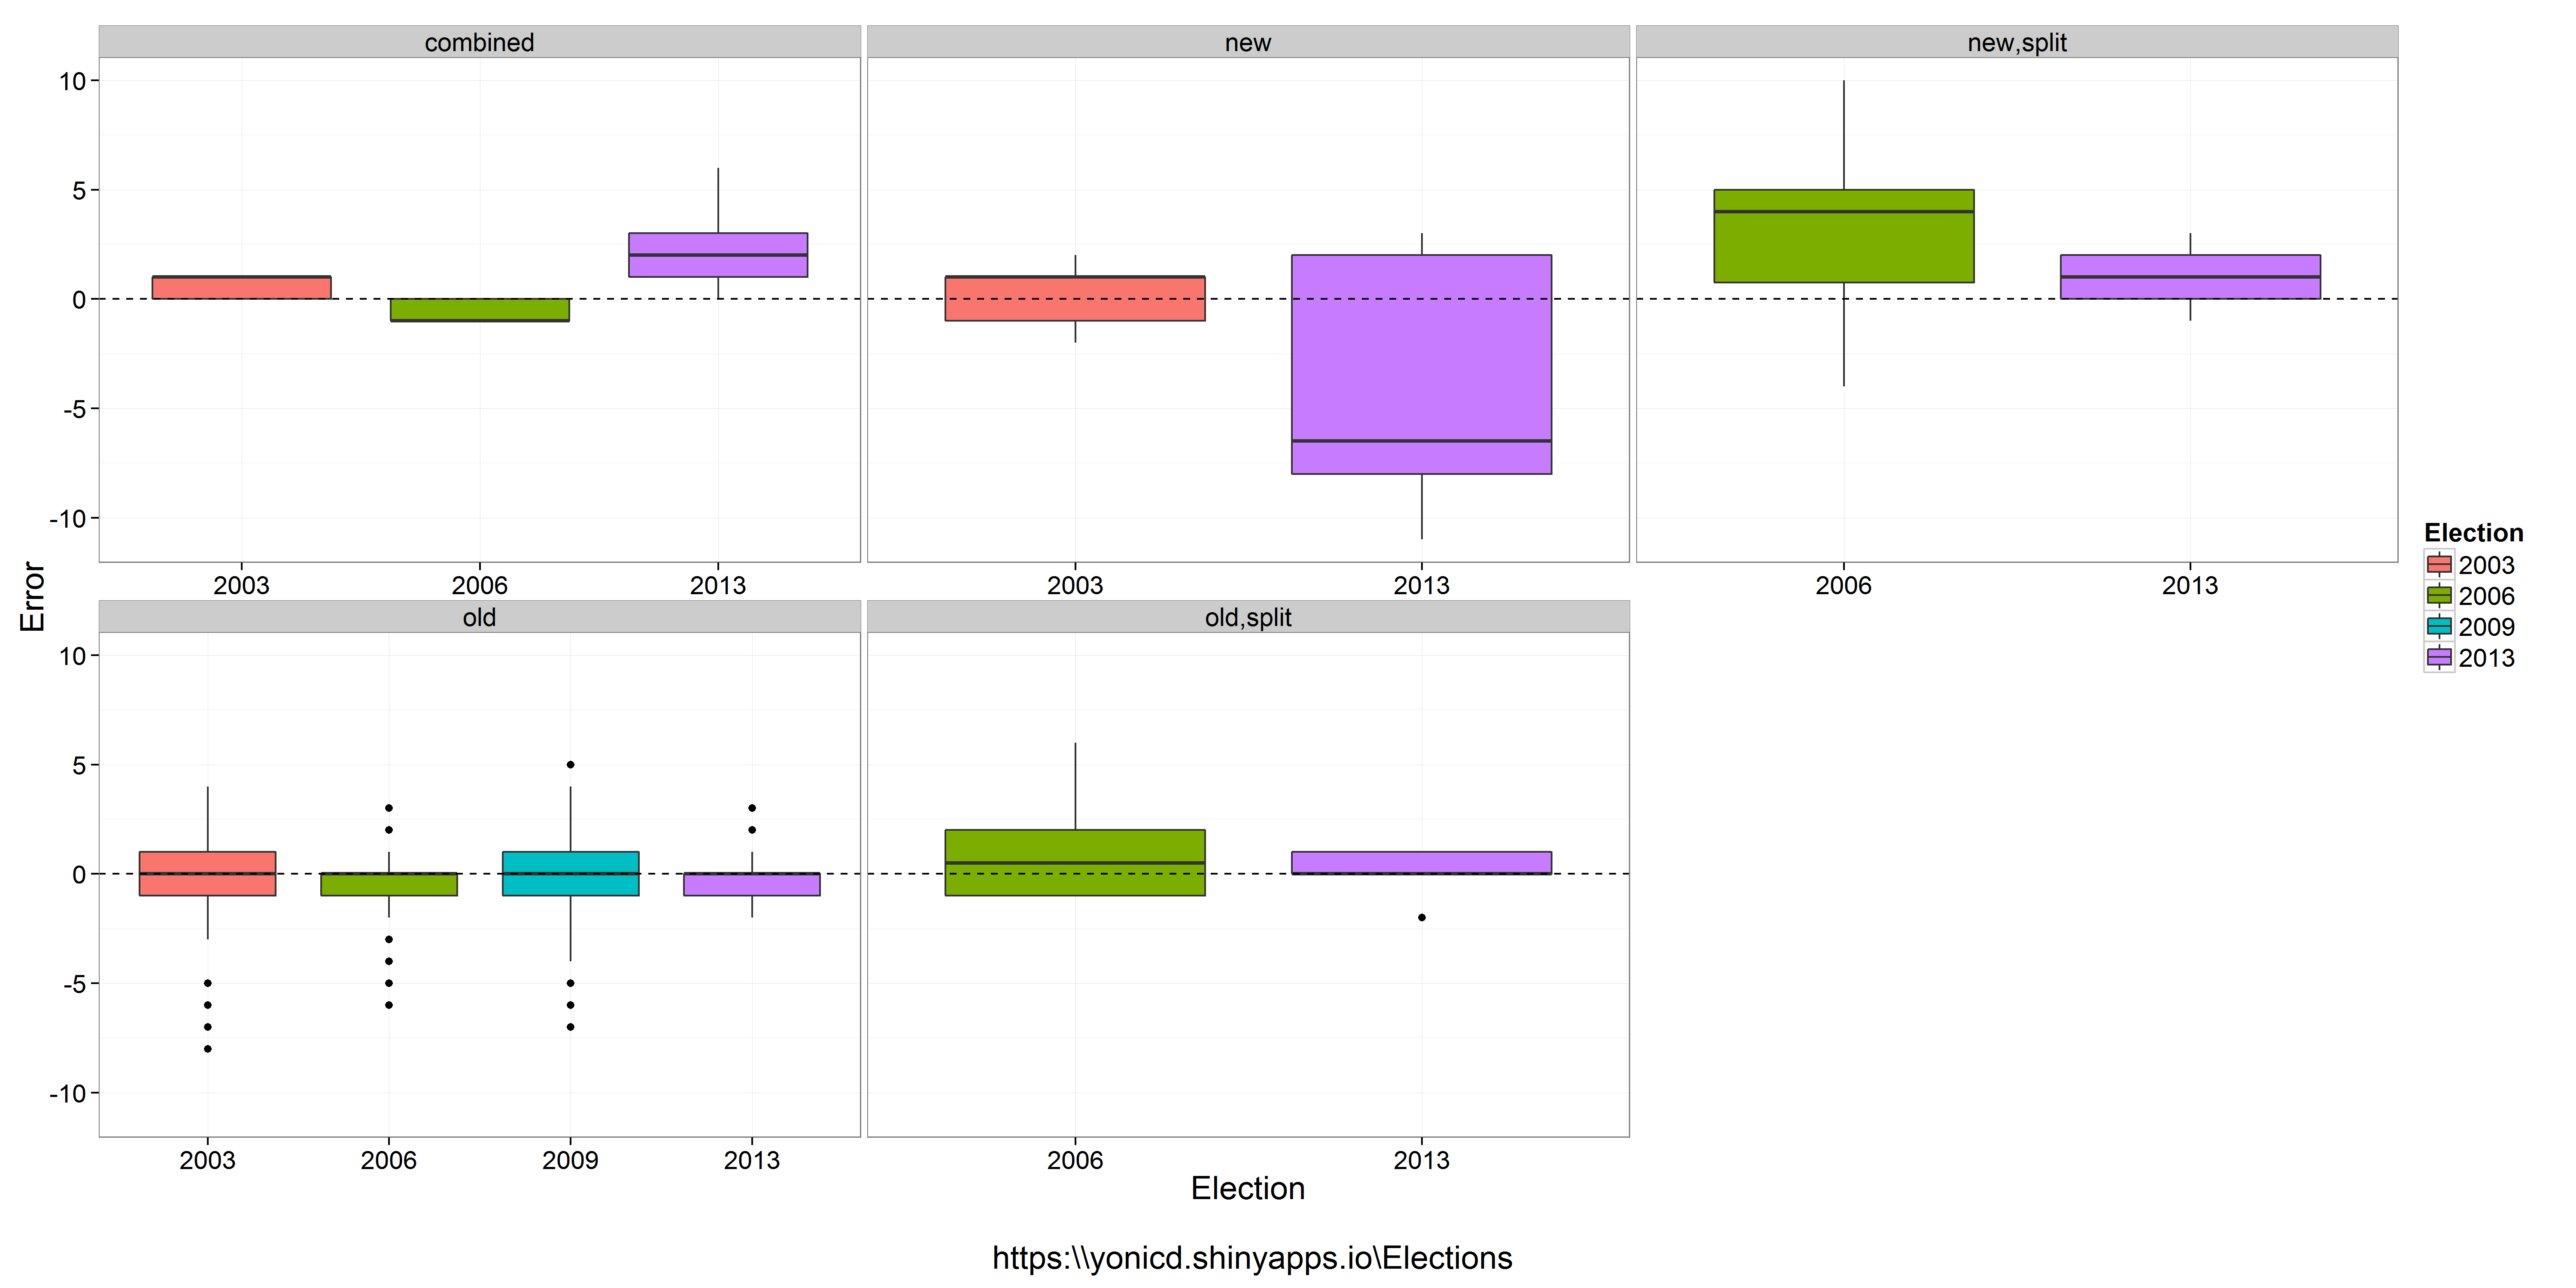
\includegraphics[width=1\linewidth]{../www/ElectionPlot_longitudinal}					\label{fig:ElectionPlot_longitudinal}
%				\end{figure}
%\begin{block}{}
%Compare party outcomes or pollster errors across elections
%\end{block}
%\end{frame}


%\subsection{Advanced Controls}
%\begin{frame}{R User console}
%\begin{figure}				
%					\centering
%					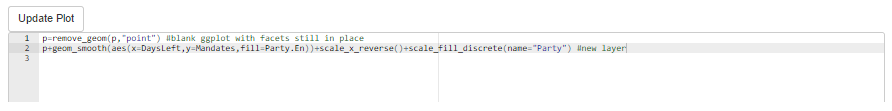
\includegraphics[width=1\linewidth]{../www/AceConsole}
%					\label{fig:ace}
%				\end{figure}
%			\begin{block}{}
%R users can control graphs through a console to add or remove ggplot2 layers and go beyond the original user interface
%			\end{block}
%\end{frame}

\section{Simulator}
\begin{frame}{Mandate Simulator}
			\begin{block}{}
			Party mandate distributions are simulated via published sampling error, mandate surplus agreements and the mandate threshold limit
			\end{block}
\begin{figure}				
					\centering
					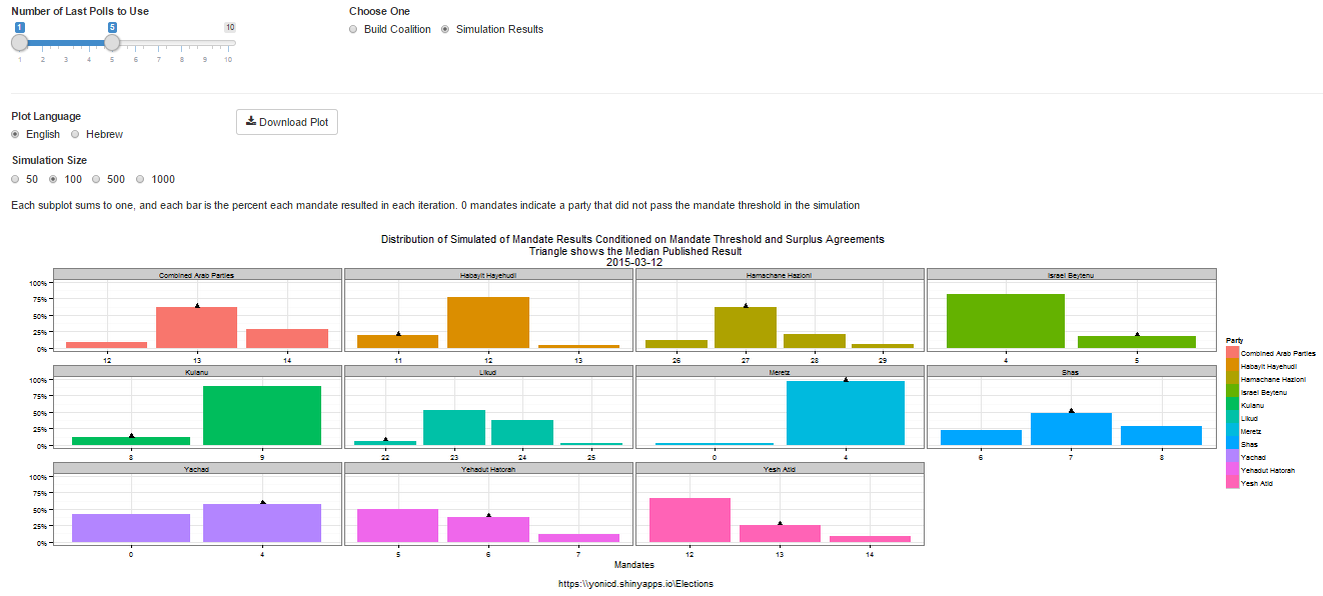
\includegraphics[width=1\linewidth]{../www/sim_screen_grab}
					\label{fig:sim_screen_grab}
				\end{figure}

\end{frame}


\section{User Generated Coalitions}
\begin{frame}{Coalition White board}
\begin{block}{}
Create coalitions based on either the simulated distribution or actual published polls and see who can pass 60 mandates
\end{block}
	\begin{figure}[h]
					\centering
					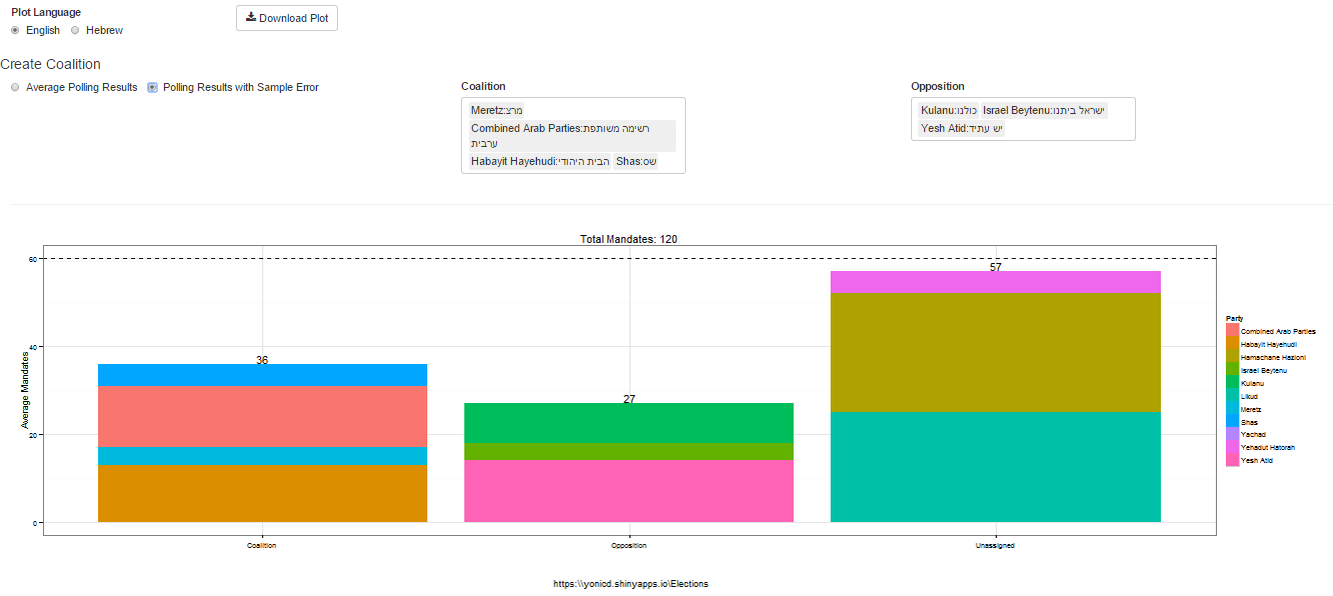
\includegraphics[width=1\linewidth]{../www/coal_screen_grab}
					\label{fig:coal_screen_grab}
	\end{figure}
\end{frame}

\begin{frame}
\centering
{\LARGE Thank You} \\

\vspace{2cm}

To visit the site and try the application

	\begin{figure}[h]
					\centering
					
\includegraphics[width=.1\linewidth]{../www/PADqr}
					\label{fig:QR}
	\end{figure}
\end{frame}

\end{document}